
\chapter{Case study: the \tth analysis application}
\label{app}

The computing resources related to all CERN projects are organized in a tier hierarchy. The first is the Tier-0 computing clusters at CERN, which from there the data is distributed to the 10 Tier-1 data centers, spread among different countries. These Tier-1 data centers are used for central processing, reconstruction of events data and Monte Carlo simulations. Tier-2 sites are dedicated to further processing and reconstruction of data and Monte Carlo events, while Tier-3 sites are used to perform data analysis and simulation \cite{LIP:Ibergrid}.

\begin{figure}[!htp]
	\begin{center}
		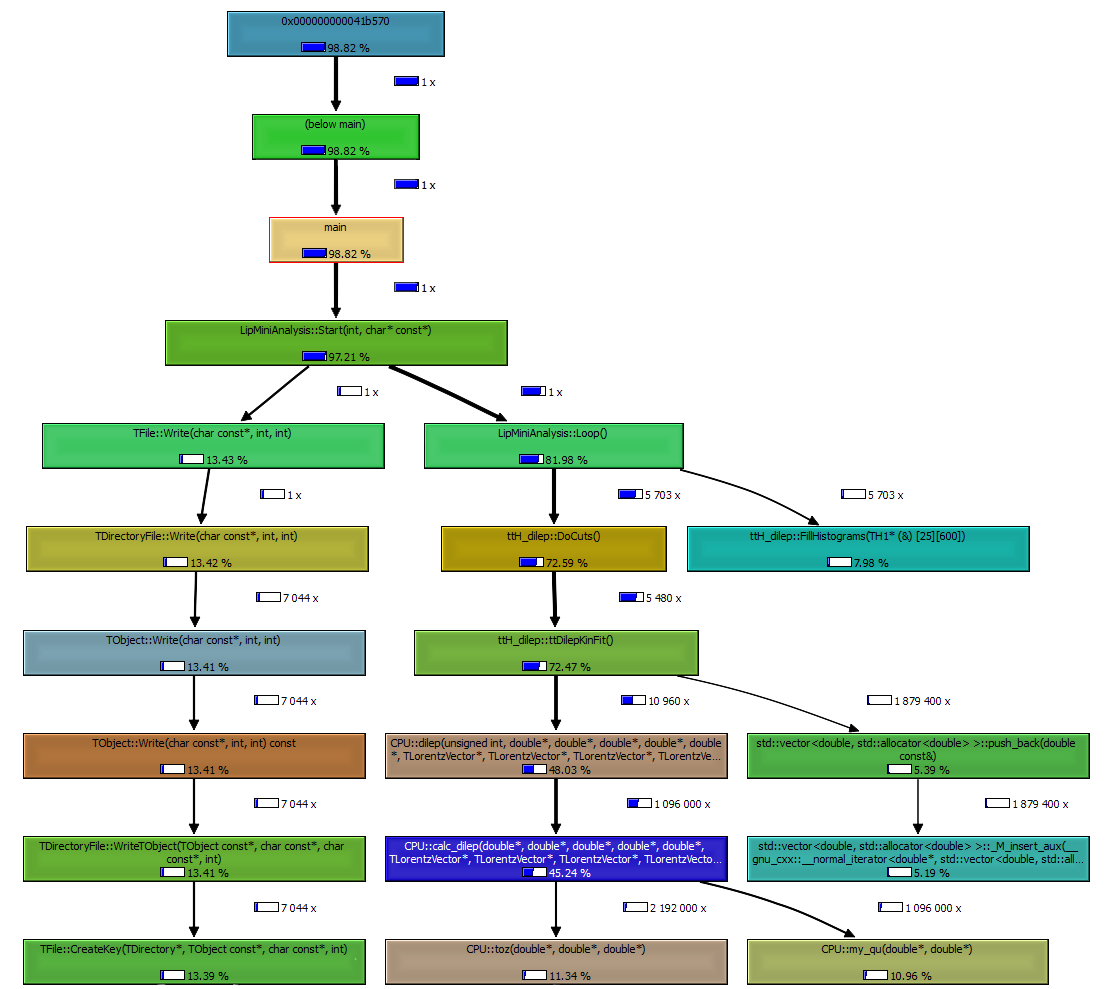
\includegraphics[scale=0.6]{../../common/img/callgraph_O3_100dilep.png}
		\caption{Callgraph generated using the Valgrind tool \cite{Callgrind} for the \tth analysis with 100 \dilep executions per event.}
		\label{fig:callgraph}
	\end{center}
\end{figure}

It is in this Tier-3 that the \tth analysis application fits. It was developed by the LIP researchers to solve the problem presented in the section \ref{context}. The application has two main dependencies: the ROOT framework \cite{CERN:ROOT} and the LipMiniAnalysis library.

The ROOT framework is being developed by CERN and provides a set of functionalities needed to handle and analyze large amounts of data. They range from data storage, in the standard formats used by CERN, to histograming, curve fitting minimization and visualization methods. It aims to provide the programmer a set of tools that will ease the development of their analysis code.

The LipMiniAnalysis is a library developed by LIP, containing a set of methods and functionalities useful for the analysis that they conduct with the ATLAS detector data. It is also prepared to read a more refined set of data resultant from the data that arrives at the Tier-3.

As illustrated by the callgraph of the analysis application in figure \ref{fig:callgraph}, the main flow of the application is controlled by the \ttLoop method. This method will apply the DoCuts function to every event to process. The event passes a series of tests and evaluations (cuts). If an event reaches the cut 20, of a total of 21, the \ttDilepKinFit function is called. It is in this function that the \ttbar and Higgs reconstructions are performed. In the beginning of the \ttDilepKinFit method, the available jets are combined two by two, as well as the leptons, as explained in section 2.

The \dilep function, called within the \ttDilepKinFit method, analytically determines the neutrinos characteristics for each jet/lepton combination, reconstructing the \ttbar system. The function is very compute intensive, as it analytically solves a system of 6 complex equations. Based on the equations result, it can produce two to four possible solutions (resulting particles). While it is compute bound, memory transfers of the required data for each time an event is processed can be a limiting factor when using accelerators. It may only become viable if the amount of \dilep executions within an event is capable of hiding the memory transfer latency. These results are used in the remaining of the \ttDilepKinFit to estimate the probability of the reconstruction, as well as reconstruct the Higgs boson. The final probability of the reconstruction is determined by combining the probability of the \ttbar reconstruction with the computed probability of the Higgs reconstruction.

As seen from the callgraph, most of the application execution time is spent in the \ttDilepKinFit method, so it is the section of the application where most efforts for optimizating the code must be focused. The rest of the functions are mainly auxiliary and I/O methods.

\newpage
